\documentclass[12pt]{article}
\usepackage{fancyhdr}
\usepackage{amsmath,amsfonts,enumerate}
\usepackage{color,graphicx}
\usepackage{tikz}
\usepackage{pgfplots}
\usepackage{listings}
\usepackage{algorithm}
\usepackage{algorithmic}
\usetikzlibrary{arrows,positioning,shapes,calc,matrix}
\pagestyle{fancy}

% Define colors for answers
\definecolor{answercolor}{RGB}{0,100,0}
\definecolor{explanationcolor}{RGB}{0,0,139}

% Custom commands for answers
\newcommand{\answer}[1]{{\color{answercolor}\textbf{Answer:} #1}}
\newcommand{\explanation}[1]{{\color{explanationcolor}#1}}

%%%%%%%%%%%%%%%%%%%%%%%%%%%%%%%%%%%%%%%%%%%%%%%%%
% Course customization based on university sources
%%%%%%%%%%%%%%%%%%%%%%%%%%%%%%%%%%%%%%%%%%%%%%%%%
\newcommand{\masunitnumber}{CENG 403}
\newcommand{\examdate}{January 2025}
\newcommand{\academicyear}{2024-2025}
\newcommand{\semester}{I}
\newcommand{\coursename}{Deep Learning - CNN Architectures \& RNN Introduction (University Sources) - ANSWERED}
\newcommand{\numberofhours}{3}
%%%%%%%%%%%%%%%%%%%%%%%%%%%%%%%%%%%%%%%%%%%%%%%%%
% CUSTOM SPACING COMMANDS FOR ANSWER SPACES
%%%%%%%%%%%%%%%%%%%%%%%%%%%%%%%%%%%%%%%%%%%%%%%%%
\newcommand{\answerspace}[1]{\vspace{#1}}
\newcommand{\questionspace}{\vspace{3cm}}        
\newcommand{\subquestionspace}{\vspace{2.5cm}}   
\newcommand{\shortanswer}{\vspace{2cm}}          
\newcommand{\mediumanswer}{\vspace{3cm}}         
\newcommand{\longanswer}{\vspace{4cm}}           
\newcommand{\journalspace}{\vspace{4.5cm}}       
\newcommand{\codespace}{\vspace{5cm}}            
%%%%%%%%%%%%%%%%%%%%%%%%%%%%%%%%%%%%%%%%%%%%%%%%%
% Header setup
%%%%%%%%%%%%%%%%%%%%%%%%%%%%%%%%%%%%%%%%%%%%%%%%%
\lhead{}
\rhead{}
\chead{{\bf MIDDLE EAST TECHNICAL UNIVERSITY}}
\lfoot{}
\rfoot{}
\cfoot{}
\begin{document}
\setlength{\headsep}{5truemm}
\setlength{\headheight}{14.5truemm}
\setlength{\voffset}{-0.45truein}
\renewcommand{\headrulewidth}{0.0pt}
\begin{center}
SEMESTER \semester\ EXAMINATION \academicyear
\end{center}
\begin{center}
{\bf \masunitnumber\ -- \coursename}
\end{center}
\vspace{20truemm}
\noindent \examdate\hspace{45truemm} TIME ALLOWED: \numberofhours\ HOURS
\vspace{19truemm}
\hrule
\vspace{19truemm}
\noindent\underline{INSTRUCTIONS TO CANDIDATES}
\vspace{8truemm}
%%%%%%%%%%%%%%%%%%%%%%%%%%%%%%%%%%%%%%%%%%%%%%%%%%%%%%
% Instructions based on university standards
%%%%%%%%%%%%%%%%%%%%%%%%%%%%%%%%%%%%%%%%%%%%%%%%%%%%%%
\begin{enumerate}
\item This examination paper contains {\bf SEVEN (7)} questions and comprises 
{\bf TEN (10)} printed pages.
\item Answer all questions. 
The marks for each question are indicated at the beginning of each question.
\item Answer each question beginning on a {\bf FRESH} page of the answer book.
\item This {\bf IS NOT an OPEN BOOK} exam.
\item Show all mathematical derivations clearly with proper notation.
\item For architectural diagrams, draw clear and labeled components.
\item Calculate all requested parameters and show intermediate steps.
\item Explain computational complexity where requested.
\end{enumerate}
%%%%%%%%%%%%%%%%%%%%%%%%%%%%%%%%%%%%%%%%%%%%%%%%%
% New page for questions
%%%%%%%%%%%%%%%%%%%%%%%%%%%%%%%%%%%%%%%%%%%%%%%%%
\newpage
\lhead{}
\rhead{\masunitnumber}
\chead{}
\lfoot{}
\cfoot{\thepage}
\rfoot{}
\setlength{\footskip}{45pt}
%%%%%%%%%%%%%%%%%%%%%%%%%%%%%%%%%%%%%%%%%%%%%%%%%%
% EXAM QUESTIONS BASED ON UNIVERSITY SOURCES
%%%%%%%%%%%%%%%%%%%%%%%%%%%%%%%%%%%%%%%%%%%%%%%%%%

\paragraph{Question 1. CNN Architectural Fundamentals and Calculations}\hfill (25 marks)\\
Based on D2L.ai and university CNN course materials covering computational aspects.

\begin{enumerate}[(a)]
    \item For a convolutional layer with the following specifications, calculate the output dimensions and number of parameters: \hfill (12 marks)
    \begin{itemize}
        \item Input: 224×224×3 RGB image
        \item 64 filters of size 7×7
        \item Stride: 2
        \item Padding: 3
        \item Bias terms included
    \end{itemize}
    
    Show all calculations including:
    \begin{itemize}
        \item Output height and width
        \item Total number of parameters
        \item Memory requirements for storing activations
    \end{itemize}
    
    \answer{Output dimensions: 112×112×64; Parameters: 9,472; Memory: 3.1 MB}
    
    \explanation{
    \textbf{Step-by-Step Calculations:}
    
    \textbf{1. Output Dimensions:}
    Using the formula: $\text{Output size} = \frac{\text{Input size} + 2 \times \text{Padding} - \text{Filter size}}{\text{Stride}} + 1$
    
    \textbf{Width calculation:}
    $$W_{out} = \frac{224 + 2 \times 3 - 7}{2} + 1 = \frac{224 + 6 - 7}{2} + 1 = \frac{223}{2} + 1 = 111.5 + 1 = 112$$
    
    \textbf{Height calculation:}
    $$H_{out} = \frac{224 + 2 \times 3 - 7}{2} + 1 = 112 \text{ (same as width)}$$
    
    \textbf{Output channels:} 64 (number of filters)
    
    \textbf{Final output dimensions:} $112 \times 112 \times 64$
    
    \textbf{2. Parameter Count:}
    \begin{itemize}
        \item Weight parameters per filter: $7 \times 7 \times 3 = 147$ (filter size × input channels)
        \item Total weight parameters: $147 \times 64 = 9,408$ (per filter × number of filters)
        \item Bias parameters: $64$ (one per filter)
        \item Total parameters: $9,408 + 64 = 9,472$
    \end{itemize}
    
    \textbf{3. Memory Requirements:}
    Assuming 32-bit floating point (4 bytes per value):
    \begin{itemize}
        \item Activation memory: $112 \times 112 \times 64 \times 4 = 3,211,264$ bytes $\approx 3.1$ MB
        \item Parameter memory: $9,472 \times 4 = 37,888$ bytes $\approx 37$ KB
        \item Total memory for this layer: $\approx 3.1$ MB (dominated by activations)
    \end{itemize}
    }
    
    \item Explain the difference between "Valid Padding" and "Same Padding" in CNNs. For a 12×12 input with a 3×3 filter and stride 1: \hfill (8 marks)
    \begin{itemize}
        \item Calculate output size with valid padding
        \item Calculate padding needed for same padding
        \item Discuss trade-offs between the two approaches
    \end{itemize}
    
    \answer{Valid padding: 10×10 output; Same padding: requires 1-pixel padding for 12×12 output}
    
    \explanation{
    \textbf{Valid Padding (No Padding):}
    \begin{itemize}
        \item Padding = 0
        \item Output size: $\frac{12 + 2(0) - 3}{1} + 1 = \frac{9}{1} + 1 = 10$
        \item Output dimensions: $10 \times 10$
        \item Filter only applied where it completely fits within input
    \end{itemize}
    
    \textbf{Same Padding:}
    \begin{itemize}
        \item Goal: Output size = Input size when stride = 1
        \item Required output: $12 \times 12$
        \item To achieve this: $12 = \frac{12 + 2p - 3}{1} + 1$
        \item Solving: $11 = 12 + 2p - 3$, so $2p = 2$, thus $p = 1$
        \item Padding needed: 1 pixel on each side
        \item Output dimensions: $12 \times 12$
    \end{itemize}
    
    \textbf{Trade-offs:}
    
    \textbf{Valid Padding Advantages:}
    \begin{itemize}
        \item No artificial padding values introduced
        \item Faster computation (smaller output)
        \item Clear semantic meaning (only real data processed)
    \end{itemize}
    
    \textbf{Valid Padding Disadvantages:}
    \begin{itemize}
        \item Output shrinks with each layer
        \item Edge information lost progressively
        \item Limited network depth before spatial dimensions become too small
    \end{itemize}
    
    \textbf{Same Padding Advantages:}
    \begin{itemize}
        \item Preserves spatial dimensions
        \item Enables deeper networks
        \item Better preservation of edge information
        \item More flexible architecture design
    \end{itemize}
    
    \textbf{Same Padding Disadvantages:}
    \begin{itemize}
        \item Introduces artificial zero values
        \item Slightly more computation
        \item May learn biases related to padding
    \end{itemize}
    }
    
    \item Compare parameter sharing in CNNs versus fully connected networks. For an image of size 256×256×3, calculate the number of parameters needed for: \hfill (5 marks)
    \begin{itemize}
        \item First layer as fully connected (to 512 units)
        \item First layer as convolutional (64 filters, 5×5)
        \item Explain the computational advantage
    \end{itemize}
    
    \answer{Fully connected: 100M+ parameters; Convolutional: 4,864 parameters - dramatic reduction through parameter sharing}
    
    \explanation{
    \textbf{Fully Connected Layer:}
    \begin{itemize}
        \item Input neurons: $256 \times 256 \times 3 = 196,608$
        \item Output neurons: $512$
        \item Weight parameters: $196,608 \times 512 = 100,663,296$
        \item Bias parameters: $512$
        \item Total parameters: $100,663,808$ $\approx 100.7$ million
    \end{itemize}
    
    \textbf{Convolutional Layer:}
    \begin{itemize}
        \item Filter size: $5 \times 5 \times 3 = 75$ weights per filter
        \item Number of filters: $64$
        \item Weight parameters: $75 \times 64 = 4,800$
        \item Bias parameters: $64$ (one per filter)
        \item Total parameters: $4,864$
    \end{itemize}
    
    \textbf{Parameter Reduction:}
    $$\text{Reduction factor} = \frac{100,663,808}{4,864} \approx 20,690$$
    
    \textbf{Computational Advantages of CNNs:}
    
    \textbf{1. Parameter Efficiency:}
    \begin{itemize}
        \item Same filter applied across entire spatial dimension
        \item Dramatic reduction in parameters ($\sim 20,000\times$ in this example)
        \item Scalable to larger images without parameter explosion
    \end{itemize}
    
    \textbf{2. Translation Invariance:}
    \begin{itemize}
        \item Features detected regardless of spatial location
        \item Natural for image processing tasks
        \item Reduces overfitting through shared representations
    \end{itemize}
    
    \textbf{3. Memory and Computational Benefits:}
    \begin{itemize}
        \item Fewer parameters to store and update
        \item More efficient gradient computations
        \item Better cache locality in hardware implementations
        \item Enables deployment on resource-constrained devices
    \end{itemize}
    }
\end{enumerate}

\newpage
\paragraph{Question 2. ResNet Architecture and Skip Connections}\hfill (30 marks)\\
Based on university deep learning courses and D2L.ai educational content.

\begin{enumerate}[(a)]
    \item Explain the mathematical foundation of residual learning. Given a target function $H(x)$, derive why learning the residual mapping $F(x) = H(x) - x$ is easier than learning $H(x)$ directly. \hfill (10 marks)
    
    Include discussion of:
    \begin{itemize}
        \item Identity function learning difficulty
        \item Gradient flow advantages
        \item Why zero functions are easier to learn
    \end{itemize}
    
    \answer{Learning residual $F(x) = H(x) - x$ is easier because when optimal mapping is close to identity, $F(x) \approx 0$, which is easier to learn than directly approximating identity through multiple nonlinear layers.}
    
    \explanation{
    \textbf{Mathematical Foundation:}
    
    \textbf{Problem with Direct Learning:}
    Given target function $H(x)$, traditional networks must learn:
    $$y = H(x)$$
    
    When optimal function is close to identity ($H(x) \approx x$), networks struggle because:
    \begin{itemize}
        \item Identity function is hard to approximate through stacked nonlinearities
        \item Multiple ReLU + linear layers cannot easily represent $f(x) = x$
        \item Small deviations from identity are difficult to learn precisely
    \end{itemize}
    
    \textbf{Residual Learning Approach:}
    Instead of learning $H(x)$ directly, learn residual:
    $$F(x) = H(x) - x$$
    
    Then the output becomes:
    $$y = F(x) + x = H(x) - x + x = H(x)$$
    
    \textbf{Why This is Easier:}
    
    \textbf{1. Zero Function Learning:}
    \begin{itemize}
        \item When $H(x) \approx x$, then $F(x) \approx 0$
        \item Zero function is much easier to learn than identity
        \item Network can achieve good performance with $F(x) = 0$ (weights near zero)
        \item Any improvement requires learning only the \textit{deviation} from identity
    \end{itemize}
    
    \textbf{2. Gradient Flow Advantages:}
    Gradient computation:
    $$\frac{\partial y}{\partial x} = \frac{\partial F(x)}{\partial x} + \frac{\partial x}{\partial x} = \frac{\partial F(x)}{\partial x} + 1$$
    
    \begin{itemize}
        \item The "+1" term ensures gradient never vanishes
        \item Even if $\frac{\partial F(x)}{\partial x} \to 0$, gradient magnitude remains $\geq 1$
        \item Provides highway for gradient flow in deep networks
    \end{itemize}
    
    \textbf{3. Optimization Landscape:}
    \begin{itemize}
        \item Identity mapping provides a strong baseline
        \item Network can only improve from this baseline
        \item Smoother loss surface around identity manifold
        \item Better conditioning for optimization algorithms
    \end{itemize}
    }
    
    \item Design and draw a complete ResNet basic block showing: \hfill (12 marks)
    \begin{itemize}
        \item Two 3×3 convolutional layers
        \item Skip connection implementation
        \item Activation function placement
        \item Dimension matching considerations
    \end{itemize}
    
    Compare this with a bottleneck block design (1×1, 3×3, 1×1 structure).
    
    \begin{center}
    \begin{tikzpicture}[scale=0.8]
        % Basic Block
        \node[align=center, font=\textbf] at (3,9) {ResNet Basic Block};
        
        % Input
        \node[draw, rectangle, minimum width=2cm, minimum height=0.8cm] (input) at (0,7) {Input $x$};
        
        % Main path
        \node[draw, rectangle, minimum width=2cm, minimum height=0.8cm] (conv1) at (0,5.5) {3×3 Conv};
        \node[draw, rectangle, minimum width=1.5cm, minimum height=0.6cm] (bn1) at (0,4.5) {BatchNorm};
        \node[draw, rectangle, minimum width=1.5cm, minimum height=0.6cm] (relu1) at (0,3.5) {ReLU};
        \node[draw, rectangle, minimum width=2cm, minimum height=0.8cm] (conv2) at (0,2.5) {3×3 Conv};
        \node[draw, rectangle, minimum width=1.5cm, minimum height=0.6cm] (bn2) at (0,1.5) {BatchNorm};
        
        % Skip connection
        \draw[thick, blue, ->] (input.east) -- (3,7) -- (3,0.8) -- (1.5,0.8);
        
        % Addition
        \node[draw, circle, minimum size=0.8cm] (add) at (1.5,0.8) {$+$};
        
        % Final ReLU
        \node[draw, rectangle, minimum width=1.5cm, minimum height=0.6cm] (relu_final) at (3,0.8) {ReLU};
        
        % Output
        \node[draw, rectangle, minimum width=2cm, minimum height=0.8cm] (output_basic) at (4.5,0.8) {Output};
        
        % Connections
        \draw[thick, ->] (input) -- (conv1);
        \draw[thick, ->] (conv1) -- (bn1);
        \draw[thick, ->] (bn1) -- (relu1);
        \draw[thick, ->] (relu1) -- (conv2);
        \draw[thick, ->] (conv2) -- (bn2);
        \draw[thick, ->] (bn2) -- (add);
        \draw[thick, ->] (add) -- (relu_final);
        \draw[thick, ->] (relu_final) -- (output_basic);
        
        % Bottleneck Block
        \node[align=center, font=\textbf] at (11,9) {ResNet Bottleneck Block};
        
        % Input
        \node[draw, rectangle, minimum width=2cm, minimum height=0.8cm] (input_bn) at (8,7) {Input $x$};
        
        % Bottleneck path
        \node[draw, rectangle, minimum width=2cm, minimum height=0.8cm] (conv1_bn) at (8,6) {1×1 Conv};
        \node[draw, rectangle, minimum width=1.5cm, minimum height=0.6cm] (bn1_bn) at (8,5.2) {BatchNorm};
        \node[draw, rectangle, minimum width=1.5cm, minimum height=0.6cm] (relu1_bn) at (8,4.4) {ReLU};
        
        \node[draw, rectangle, minimum width=2cm, minimum height=0.8cm] (conv2_bn) at (8,3.6) {3×3 Conv};
        \node[draw, rectangle, minimum width=1.5cm, minimum height=0.6cm] (bn2_bn) at (8,2.8) {BatchNorm};
        \node[draw, rectangle, minimum width=1.5cm, minimum height=0.6cm] (relu2_bn) at (8,2) {ReLU};
        
        \node[draw, rectangle, minimum width=2cm, minimum height=0.8cm] (conv3_bn) at (8,1.2) {1×1 Conv};
        \node[draw, rectangle, minimum width=1.5cm, minimum height=0.6cm] (bn3_bn) at (8,0.4) {BatchNorm};
        
        % Skip connection for bottleneck
        \draw[thick, blue, ->] (input_bn.east) -- (11,7) -- (11,-0.4) -- (9.5,-0.4);
        
        % Addition for bottleneck
        \node[draw, circle, minimum size=0.8cm] (add_bn) at (9.5,-0.4) {$+$};
        
        % Final ReLU for bottleneck
        \node[draw, rectangle, minimum width=1.5cm, minimum height=0.6cm] (relu_final_bn) at (11,-0.4) {ReLU};
        
        % Output for bottleneck
        \node[draw, rectangle, minimum width=2cm, minimum height=0.8cm] (output_bn) at (12.5,-0.4) {Output};
        
        % Connections for bottleneck
        \draw[thick, ->] (input_bn) -- (conv1_bn);
        \draw[thick, ->] (conv1_bn) -- (bn1_bn);
        \draw[thick, ->] (bn1_bn) -- (relu1_bn);
        \draw[thick, ->] (relu1_bn) -- (conv2_bn);
        \draw[thick, ->] (conv2_bn) -- (bn2_bn);
        \draw[thick, ->] (bn2_bn) -- (relu2_bn);
        \draw[thick, ->] (relu2_bn) -- (conv3_bn);
        \draw[thick, ->] (conv3_bn) -- (bn3_bn);
        \draw[thick, ->] (bn3_bn) -- (add_bn);
        \draw[thick, ->] (add_bn) -- (relu_final_bn);
        \draw[thick, ->] (relu_final_bn) -- (output_bn);
        
        % Labels
        \node[blue] at (4.5,7) {\textbf{Skip Connection}};
        \node[red] at (0,-1) {\textbf{$F(x) + x$}};
        \node[red] at (8,-2) {\textbf{Reduces parameters}};
    \end{tikzpicture}
    \end{center}
    
    \explanation{
    \textbf{Basic Block Design:}
    \begin{itemize}
        \item \textbf{Structure:} Conv3×3 → BatchNorm → ReLU → Conv3×3 → BatchNorm → Add → ReLU
        \item \textbf{Skip Connection:} Direct addition of input to processed output
        \item \textbf{Activation Placement:} ReLU after each BatchNorm, final ReLU after addition
        \item \textbf{Parameters:} If input has $C$ channels: $2 \times (3 \times 3 \times C \times C) = 18C^2$
    \end{itemize}
    
    \textbf{Bottleneck Block Design:}
    \begin{itemize}
        \item \textbf{Structure:} Conv1×1 → BN → ReLU → Conv3×3 → BN → ReLU → Conv1×1 → BN → Add → ReLU
        \item \textbf{Purpose:} Reduce parameters while maintaining representational capacity
        \item \textbf{Mechanism:} 1×1 convolutions reduce/expand channels, 3×3 works on reduced dimensions
        \item \textbf{Example:} Input 256 channels → 64 channels → 64 channels → 256 channels
        \item \textbf{Parameters:} $256 \times 64 + 3 \times 3 \times 64 \times 64 + 64 \times 256 = 69,632$ vs. $3 \times 3 \times 256 \times 256 = 589,824$ for basic block
    \end{itemize}
    
    \textbf{Dimension Matching:}
    \begin{itemize}
        \item When input and output dimensions match: direct addition
        \item When dimensions differ (stride 2, channel change): use 1×1 conv on skip connection
        \item Skip connection projection: $x' = W_s x$ where $W_s$ is 1×1 convolution
    \end{itemize}
    }
    
    \item Analyze gradient flow in ResNet vs. vanilla deep networks. For a 50-layer network, explain mathematically why ResNet can avoid vanishing gradients. \hfill (8 marks)
    
    Include:
    \begin{itemize}
        \item Gradient computation through skip connections
        \item Comparison with traditional deep networks
        \item Why identity mappings preserve gradient magnitude
    \end{itemize}
    
    \answer{ResNet avoids vanishing gradients because skip connections provide identity paths where $\frac{\partial y}{\partial x} = 1 + \frac{\partial F(x)}{\partial x}$, ensuring gradient magnitude never falls below 1, unlike vanilla networks where gradients multiply through all layers.}
    
    \explanation{
    \textbf{Gradient Flow in Vanilla Networks:}
    
    For a 50-layer network: $y = f_{50}(f_{49}(\ldots f_2(f_1(x)) \ldots))$
    
    Gradient computation using chain rule:
    $$\frac{\partial L}{\partial x} = \frac{\partial L}{\partial y} \prod_{i=1}^{50} \frac{\partial f_i}{\partial x_i}$$
    
    \textbf{Problems:}
    \begin{itemize}
        \item Each $\frac{\partial f_i}{\partial x_i}$ typically $< 1$ for saturating activations
        \item Product of 50 terms $< 1$ leads to exponential decay
        \item For sigmoid: $\max(\sigma'(x)) = 0.25$, so gradient can shrink by factor $(0.25)^{50} \approx 10^{-30}$
    \end{itemize}
    
    \textbf{Gradient Flow in ResNet:}
    
    For ResNet block: $y = F(x) + x$
    
    Gradient computation:
    $$\frac{\partial y}{\partial x} = \frac{\partial F(x)}{\partial x} + \frac{\partial x}{\partial x} = \frac{\partial F(x)}{\partial x} + 1$$
    
    \textbf{Through entire network:}
    $$\frac{\partial L}{\partial x} = \frac{\partial L}{\partial y} \prod_{i=1}^{N} \left( \frac{\partial F_i(x_i)}{\partial x_i} + 1 \right)$$
    
    \textbf{Key Advantages:}
    
    \textbf{1. Gradient Lower Bound:}
    \begin{itemize}
        \item Even if $\frac{\partial F(x)}{\partial x} \to 0$, we have $\frac{\partial y}{\partial x} = 1$
        \item Gradient magnitude is always $\geq 1$ for each block
        \item No exponential decay through depth
    \end{itemize}
    
    \textbf{2. Multiple Gradient Paths:}
    \begin{itemize}
        \item Direct path through skip connections (always magnitude 1)
        \item Processed paths through weight layers
        \item Gradients can flow through whichever path is most effective
    \end{itemize}
    
    \textbf{3. Mathematical Proof of Non-Vanishing:}
    For single ResNet block:
    $$\left| \frac{\partial y}{\partial x} \right| = \left| \frac{\partial F(x)}{\partial x} + 1 \right| \geq \left| 1 - \left| \frac{\partial F(x)}{\partial x} \right| \right|$$
    
    As long as $\left| \frac{\partial F(x)}{\partial x} \right| < 1$, we have $\left| \frac{\partial y}{\partial x} \right| > 0$
    
    \textbf{Comparison Summary:}
    \begin{itemize}
        \item \textbf{Vanilla:} Gradient magnitude exponentially decreases with depth
        \item \textbf{ResNet:} Gradient magnitude maintained through identity paths
        \item \textbf{Result:} ResNet enables training of networks with 1000+ layers
    \end{itemize}
    }
\end{enumerate}

\newpage
\paragraph{Question 3. DenseNet and Advanced CNN Architectures}\hfill (22 marks)\\
Based on modern CNN architecture research and educational materials.

\begin{enumerate}[(a)]
    \item Compare DenseNet with ResNet architectures. Explain the key difference: \hfill (8 marks)
    $$\text{ResNet: } x_l = H_l(x_{l-1}) + x_{l-1}$$
    $$\text{DenseNet: } x_l = H_l([x_0, x_1, \ldots, x_{l-1}])$$
    
    Discuss advantages and disadvantages of each approach.
    
    \answer{ResNet uses element-wise addition of skip connections while DenseNet concatenates feature maps from all previous layers, creating denser connectivity but higher memory requirements.}
    
    \explanation{
    \textbf{Architectural Differences:}
    
    \textbf{ResNet Approach:}
    \begin{itemize}
        \item $x_l = H_l(x_{l-1}) + x_{l-1}$ (element-wise addition)
        \item Each layer connects to previous layer and skips one layer
        \item Fixed number of channels throughout residual blocks
        \item Additive information combination
    \end{itemize}
    
    \textbf{DenseNet Approach:}
    \begin{itemize}
        \item $x_l = H_l([x_0, x_1, \ldots, x_{l-1}])$ (concatenation)
        \item Each layer connects to ALL previous layers
        \item Growing number of input channels: $k_0 + l \times k$ channels for layer $l$
        \item Concatenative information combination
    \end{itemize}
    
    \textbf{Advantages and Disadvantages:}
    
    \begin{tabular}{|p{2.5cm}|p{5cm}|p{5cm}|}
    \hline
    & \textbf{ResNet} & \textbf{DenseNet} \\
    \hline
    \textbf{Advantages} & 
    \begin{itemize}
        \item Lower memory usage
        \item Faster training/inference
        \item Simpler implementation
        \item Good gradient flow
        \item Scalable to very deep networks
    \end{itemize} & 
    \begin{itemize}
        \item Better feature reuse
        \item Stronger gradient flow
        \item More parameter efficient
        \item Better performance on small datasets
        \item Implicit regularization
    \end{itemize} \\
    \hline
    \textbf{Disadvantages} & 
    \begin{itemize}
        \item Information loss through addition
        \item Less feature reuse
        \item May require more parameters
    \end{itemize} & 
    \begin{itemize}
        \item High memory requirements
        \item Slower due to concatenations
        \item Complex implementation
        \item Quadratic growth in connections
    \end{itemize} \\
    \hline
    \end{tabular}
    
    \textbf{When to Use Each:}
    \begin{itemize}
        \item \textbf{ResNet:} Large-scale problems, limited memory, need for speed
        \item \textbf{DenseNet:} Small datasets, parameter efficiency priority, research settings
    \end{itemize}
    }
    
    \item For a DenseNet block with 4 layers, each producing 12 feature maps (growth rate k=12), and input of 64 channels: \hfill (10 marks)
    \begin{itemize}
        \item Calculate the number of input channels for each layer
        \item Compute total memory requirements for concatenations
        \item Explain how transition layers reduce dimensionality
        \item Calculate parameters for 1×1 conv in transition layer
    \end{itemize}
    
    \answer{Layer inputs: 64, 76, 88, 100 channels; Memory grows quadratically; Transition layers use 1×1 conv for dimensionality reduction}
    
    \explanation{
    \textbf{Channel Calculation for Each Layer:}
    
    Given: Initial channels $= 64$, Growth rate $k = 12$
    
    \begin{itemize}
        \item \textbf{Layer 1:} Input channels = $64$ (initial)
        \item \textbf{Layer 2:} Input channels = $64 + 12 = 76$ (initial + layer 1 output)
        \item \textbf{Layer 3:} Input channels = $64 + 12 + 12 = 88$ (initial + layer 1 + layer 2)
        \item \textbf{Layer 4:} Input channels = $64 + 12 + 12 + 12 = 100$ (all previous layers)
    \end{itemize}
    
    \textbf{General Formula:} Layer $l$ has $k_0 + (l-1) \times k$ input channels
    
    \textbf{Memory Requirements for Concatenations:}
    
    Assuming feature maps of size $H \times W$ and 32-bit floats:
    \begin{itemize}
        \item \textbf{After Layer 1:} $(64 + 12) \times H \times W \times 4 = 76HW \times 4$ bytes
        \item \textbf{After Layer 2:} $(64 + 12 + 12) \times H \times W \times 4 = 88HW \times 4$ bytes
        \item \textbf{After Layer 3:} $(64 + 12 + 12 + 12) \times H \times W \times 4 = 100HW \times 4$ bytes
        \item \textbf{After Layer 4:} $(64 + 12 + 12 + 12 + 12) \times H \times W \times 4 = 112HW \times 4$ bytes
    \end{itemize}
    
    \textbf{Total Memory:} $(76 + 88 + 100 + 112) \times HW \times 4 = 376HW \times 4$ bytes
    
    \textbf{Transition Layers:}
    
    \textbf{Purpose:} Reduce the number of feature maps to control model complexity
    
    \textbf{Structure:}
    \begin{itemize}
        \item \textbf{1×1 Convolution:} Reduces number of channels (typically by factor of 2)
        \item \textbf{Average Pooling:} Reduces spatial dimensions (typically 2×2 with stride 2)
    \end{itemize}
    
    \textbf{Example Transition Layer:}
    \begin{itemize}
        \item Input: $112$ channels from dense block
        \item 1×1 Conv: $112 \to 56$ channels (compression factor = 0.5)
        \item 2×2 Average Pooling: $(H, W) \to (H/2, W/2)$
    \end{itemize}
    
    \textbf{Parameter Calculation for 1×1 Transition Conv:}
    \begin{itemize}
        \item Input channels: $112$
        \item Output channels: $56$ (with compression factor 0.5)
        \item Filter size: $1 \times 1$
        \item Weight parameters: $1 \times 1 \times 112 \times 56 = 6,272$
        \item Bias parameters: $56$
        \item Total parameters: $6,272 + 56 = 6,328$
    \end{itemize}
    
    \textbf{Benefits of Transition Layers:}
    \begin{itemize}
        \item Control computational complexity
        \item Reduce memory requirements
        \item Maintain model efficiency as network grows
        \item Enable deeper DenseNet architectures
    \end{itemize}
    }
    
    \item Design a Highway Network gate mechanism. Write the mathematical equations for: \hfill (4 marks)
    $$y = H(x,W_H) \cdot T(x,W_T) + x \cdot C(x,W_C)$$
    
    Explain how this differs from standard residual connections.
    
    \answer{Highway networks use learnable gates $T(x)$ and $C(x) = 1-T(x)$ to control information flow, unlike ResNet's fixed additive skip connections.}
    
    \explanation{
    \textbf{Highway Network Mathematical Formulation:}
    
    \textbf{Complete Equations:}
    \begin{align}
    T(x, W_T) &= \sigma(W_T x + b_T) \quad \text{(Transform gate)} \\
    C(x, W_C) &= 1 - T(x, W_T) \quad \text{(Carry gate)} \\
    H(x, W_H) &= \text{ReLU}(W_H x + b_H) \quad \text{(Transform function)} \\
    y &= H(x, W_H) \cdot T(x, W_T) + x \cdot C(x, W_C)
    \end{align}
    
    Where:
    \begin{itemize}
        \item $\sigma$ is the sigmoid function ensuring $T(x) \in [0,1]$
        \item $T(x)$ controls how much transformed information passes through
        \item $C(x) = 1 - T(x)$ controls how much original information passes through
        \item $T(x) + C(x) = 1$ ensures information conservation
    \end{itemize}
    
    \textbf{Differences from Standard ResNet:}
    
    \begin{tabular}{|p{5cm}|p{5cm}|}
    \hline
    \textbf{Highway Networks} & \textbf{ResNet} \\
    \hline
    $y = H(x) \cdot T(x) + x \cdot C(x)$ & $y = H(x) + x$ \\
    \hline
    Learnable, adaptive gates & Fixed additive skip \\
    \hline
    $T(x), C(x)$ are input-dependent & Skip connection always active \\
    \hline
    Multiplicative gating & Additive skip connection \\
    \hline
    Can completely block paths & Both paths always contribute \\
    \hline
    More parameters (gate weights) & Fewer parameters \\
    \hline
    Adaptive information routing & Fixed information combination \\
    \hline
    \end{tabular}
    
    \textbf{Key Advantages of Highway Networks:}
    \begin{itemize}
        \item \textbf{Adaptive Control:} Gates learn when to transform vs. preserve information
        \item \textbf{Flexible Routing:} Can dynamically choose optimal information paths
        \item \textbf{Input-Dependent Behavior:} Different inputs may use different paths
    \end{itemize}
    
    \textbf{Why ResNet Became More Popular:}
    \begin{itemize}
        \item \textbf{Simplicity:} Fixed addition is easier to implement and understand
        \item \textbf{Efficiency:} Fewer parameters and computations
        \item \textbf{Reliability:} Less complex optimization landscape
        \item \textbf{Effectiveness:} Achieved excellent results with simpler approach
    \end{itemize}
    }
\end{enumerate}

\newpage
\paragraph{Question 4. CNN Optimization and Efficiency}\hfill (20 marks)\\
Based on practical CNN implementation and optimization techniques.

\begin{enumerate}[(a)]
    \item Analyze binary neural networks for edge deployment. Given a standard CNN with: \hfill (10 marks)
    \begin{itemize}
        \item 10M parameters (32-bit floats)
        \item 50 GFLOPS for inference
    \end{itemize}
    
    Calculate:
    \begin{itemize}
        \item Memory reduction with binary weights
        \item Speed improvement estimates
        \item Accuracy trade-offs to consider
        \item When binary networks are appropriate
    \end{itemize}
    
    \answer{Memory reduction: 32×; Speed improvement: 10-30×; Accuracy loss: 5-15\%; Suitable for edge devices and real-time applications.}
    
    \explanation{
    \textbf{Memory Reduction Calculation:}
    
    \textbf{Standard CNN:}
    \begin{itemize}
        \item Parameters: 10M × 32 bits = 320M bits = 40 MB
        \item Each parameter: 32-bit float (4 bytes)
    \end{itemize}
    
    \textbf{Binary CNN:}
    \begin{itemize}
        \item Parameters: 10M × 1 bit = 10M bits = 1.25 MB
        \item Each parameter: 1 bit (±1 values)
    \end{itemize}
    
    \textbf{Memory Reduction:} $\frac{40 \text{ MB}}{1.25 \text{ MB}} = 32×$
    
    \textbf{Speed Improvement Analysis:}
    
    \textbf{Computational Changes:}
    \begin{itemize}
        \item \textbf{Standard:} Floating-point multiplications + additions
        \item \textbf{Binary:} XNOR operations + bit counting (popcount)
    \end{itemize}
    
    \textbf{Operation Comparison:}
    \begin{itemize}
        \item FP32 multiplication: ~100-200 CPU cycles
        \item XNOR + popcount: ~1-2 CPU cycles
        \item Theoretical speedup: 50-200×
        \item Practical speedup: 10-30× (due to memory access, other operations)
    \end{itemize}
    
    \textbf{Estimated Performance:}
    \begin{itemize}
        \item Original: 50 GFLOPS
        \item Binary (conservative): 50 × 10 = 500 GFLOPS equivalent
        \item Binary (optimistic): 50 × 30 = 1500 GFLOPS equivalent
    \end{itemize}
    
    \textbf{Accuracy Trade-offs:}
    
    \textbf{Typical Accuracy Loss:}
    \begin{itemize}
        \item \textbf{CIFAR-10:} 2-5\% accuracy drop
        \item \textbf{ImageNet:} 10-15\% accuracy drop
        \item \textbf{Simple tasks:} Minimal impact
        \item \textbf{Complex tasks:} Significant degradation
    \end{itemize}
    
    \textbf{Factors Affecting Accuracy:}
    \begin{itemize}
        \item Task complexity
        \item Network architecture
        \item Training methodology
        \item Binary quantization scheme
    \end{itemize}
    
    \textbf{When Binary Networks are Appropriate:}
    
    \textbf{Suitable Applications:}
    \begin{itemize}
        \item \textbf{Edge Computing:} IoT devices, mobile phones
        \item \textbf{Real-time Processing:} Video analysis, autonomous systems
        \item \textbf{Energy-Constrained:} Battery-powered devices
        \item \textbf{Simple Tasks:} Object detection, basic classification
        \item \textbf{Privacy-Critical:} On-device processing requirements
    \end{itemize}
    
    \textbf{Unsuitable Applications:}
    \begin{itemize}
        \item \textbf{High-Accuracy Required:} Medical diagnosis, scientific computing
        \item \textbf{Complex Tasks:} Fine-grained classification, segmentation
        \item \textbf{Research Applications:} Where accuracy is paramount
        \item \textbf{Cloud Computing:} Where resources are abundant
    \end{itemize}
    }
    
    \item Compare different normalization strategies in deep CNNs: \hfill (10 marks)
    \begin{itemize}
        \item Batch Normalization: benefits and limitations
        \item Why BatchNorm helps in very deep networks (10,000+ layers)
        \item Relationship between BatchNorm and gradient stability
        \item Alternative normalization methods
    \end{itemize}
    
    \answer{BatchNorm normalizes layer inputs to stabilize training, enabling very deep networks by maintaining gradient flow and reducing internal covariate shift, but has limitations with small batches and inference.}
    
    \explanation{
    \textbf{Batch Normalization Fundamentals:}
    
    \textbf{Mathematical Formulation:}
    For mini-batch $\mathcal{B} = \{x_1, x_2, \ldots, x_m\}$:
    \begin{align}
    \mu_{\mathcal{B}} &= \frac{1}{m} \sum_{i=1}^m x_i \\
    \sigma^2_{\mathcal{B}} &= \frac{1}{m} \sum_{i=1}^m (x_i - \mu_{\mathcal{B}})^2 \\
    \hat{x}_i &= \frac{x_i - \mu_{\mathcal{B}}}{\sqrt{\sigma^2_{\mathcal{B}} + \epsilon}} \\
    y_i &= \gamma \hat{x}_i + \beta
    \end{align}
    
    \textbf{Benefits of Batch Normalization:}
    
    \textbf{1. Gradient Stability:}
    \begin{itemize}
        \item Prevents gradient vanishing/exploding
        \item Normalizes gradients across layers
        \item Enables higher learning rates
    \end{itemize}
    
    \textbf{2. Reduced Internal Covariate Shift:}
    \begin{itemize}
        \item Stabilizes input distributions to each layer
        \item Reduces dependence on careful weight initialization
        \item Accelerates training convergence
    \end{itemize}
    
    \textbf{3. Regularization Effect:}
    \begin{itemize}
        \item Adds noise through batch statistics
        \item Reduces overfitting
        \item Can reduce need for Dropout
    \end{itemize}
    
    \textbf{Why BatchNorm Enables Very Deep Networks (10,000+ layers):}
    
    \textbf{1. Gradient Flow Preservation:}
    \begin{itemize}
        \item Maintains unit variance across layers
        \item Prevents gradient magnitude from shrinking/growing exponentially
        \item Each layer receives well-conditioned gradients
    \end{itemize}
    
    \textbf{2. Activation Distribution Control:}
    \begin{itemize}
        \item Keeps activations in linear region of activation functions
        \item Prevents saturation that causes gradient vanishing
        \item Maintains expressiveness throughout the network
    \end{itemize}
    
    \textbf{3. Decoupled Layer Dependencies:}
    \begin{itemize}
        \item Reduces interdependence between layer parameters
        \item Enables more independent layer-wise learning
        \item Stabilizes very deep optimization landscapes
    \end{itemize}
    
    \textbf{Relationship Between BatchNorm and Gradient Stability:}
    
    \textbf{Gradient Flow Analysis:}
    Without BatchNorm: $\frac{\partial L}{\partial x} = \frac{\partial L}{\partial y} \cdot W$
    With BatchNorm: $\frac{\partial L}{\partial x} = \frac{\partial L}{\partial y} \cdot \frac{\gamma}{\sqrt{\sigma^2 + \epsilon}}$
    
    \textbf{Key Improvements:}
    \begin{itemize}
        \item Gradient magnitude controlled by $\gamma$ (learnable)
        \item Variance normalization prevents explosion/vanishing
        \item More stable gradient flow enables deeper architectures
    \end{itemize}
    
    \textbf{Limitations of Batch Normalization:}
    
    \textbf{1. Batch Size Dependency:}
    \begin{itemize}
        \item Poor performance with small batches
        \item Batch statistics become unreliable
        \item Different behavior during training vs. inference
    \end{itemize}
    
    \textbf{2. Sequential Data Issues:}
    \begin{itemize}
        \item Difficulty with RNNs and variable-length sequences
        \item Temporal dependencies can be disrupted
    \end{itemize}
    
    \textbf{3. Inference Complications:}
    \begin{itemize}
        \item Requires running statistics from training
        \item Domain shift can affect normalization statistics
    \end{itemize}
    
    \textbf{Alternative Normalization Methods:}
    
    \textbf{1. Layer Normalization:}
    \begin{itemize}
        \item Normalizes across feature dimension instead of batch
        \item Better for RNNs and small batches
        \item $\mu_l = \frac{1}{H} \sum_{i=1}^H x_i$, $\sigma_l = \sqrt{\frac{1}{H} \sum_{i=1}^H (x_i - \mu_l)^2}$
    \end{itemize}
    
    \textbf{2. Instance Normalization:}
    \begin{itemize}
        \item Normalizes each sample independently
        \item Useful for style transfer and GANs
        \item Removes instance-specific contrast information
    \end{itemize}
    
    \textbf{3. Group Normalization:}
    \begin{itemize}
        \item Divides channels into groups for normalization
        \item Batch-size independent
        \item Good compromise between Layer and Instance normalization
    \end{itemize}
    
    \textbf{4. Weight Normalization:}
    \begin{itemize}
        \item Normalizes weight vectors instead of activations
        \item Decouples weight magnitude from direction
        \item Computational benefits for certain architectures
    \end{itemize}
    }
\end{enumerate}

\newpage
\paragraph{Question 5. RNN Fundamentals and Unfolding}\hfill (28 marks)\\
Based on sequence modeling and RNN theory from university courses.

\begin{enumerate}[(a)]
    \item Classify the following problems and suggest appropriate architectures: \hfill (8 marks)
    \begin{itemize}
        \item Image captioning
        \item Spam email detection
        \item Machine translation
        \item Real-time speech recognition
    \end{itemize}
    
    For each, specify: one-to-one, one-to-many, many-to-one, or many-to-many architecture.
    
    \answer{Image captioning: One-to-many; Spam detection: Many-to-one; Translation: Many-to-many; Speech recognition: Many-to-many}
    
    \explanation{
    \textbf{1. Image Captioning: One-to-Many}
    \begin{itemize}
        \item \textbf{Input:} Single image (one)
        \item \textbf{Output:} Sequence of words (many)
        \item \textbf{Architecture:} CNN encoder + RNN decoder
        \item \textbf{Example:} Image → "A dog playing in the park"
        \item \textbf{Implementation:} CNN extracts image features, RNN generates caption word by word
    \end{itemize}
    
    \textbf{2. Spam Email Detection: Many-to-One}
    \begin{itemize}
        \item \textbf{Input:} Sequence of words/tokens (many)
        \item \textbf{Output:} Single classification (spam/not spam) (one)
        \item \textbf{Architecture:} RNN encoder with final classification layer
        \item \textbf{Example:} "Free money click now" → Spam
        \item \textbf{Implementation:} Process email text sequentially, final hidden state feeds classifier
    \end{itemize}
    
    \textbf{3. Machine Translation: Many-to-Many (Sequence-to-Sequence)}
    \begin{itemize}
        \item \textbf{Input:} Sequence in source language (many)
        \item \textbf{Output:} Sequence in target language (many)
        \item \textbf{Architecture:} Encoder-Decoder with attention
        \item \textbf{Example:} "How are you?" → "Comment allez-vous?"
        \item \textbf{Implementation:} Encoder RNN processes source, decoder RNN generates target
    \end{itemize}
    
    \textbf{4. Real-time Speech Recognition: Many-to-Many (Synchronous)}
    \begin{itemize}
        \item \textbf{Input:} Stream of audio features (many)
        \item \textbf{Output:} Stream of text/phonemes (many)
        \item \textbf{Architecture:} Streaming RNN with CTC or attention
        \item \textbf{Example:} Audio waveform → Real-time transcription
        \item \textbf{Implementation:} Process audio frames sequentially, output text in real-time
    \end{itemize}
    
    \textbf{Architecture Design Guidelines:}
    \begin{itemize}
        \item \textbf{One-to-Many:} Use RNN decoder with initial state from encoded input
        \item \textbf{Many-to-One:} Use RNN encoder, take final hidden state for classification
        \item \textbf{Many-to-Many:} Use encoder-decoder or synchronous RNN depending on alignment
    \end{itemize}
    }
    
    \item Explain RNN unfolding process. For the recurrent equation: \hfill (12 marks)
    $$h_t = \tanh(W_{hx} x_t + W_{hh} h_{t-1} + b_h)$$
    $$y_t = W_{hy} h_t + b_y$$
    
    Draw the unfolded network for T=3 time steps showing:
    \begin{itemize}
        \item Weight sharing across time
        \item Hidden state connections
        \item How this becomes a feedforward network
        \item Why sequences of different lengths can be handled
    \end{itemize}
    
    \begin{center}
    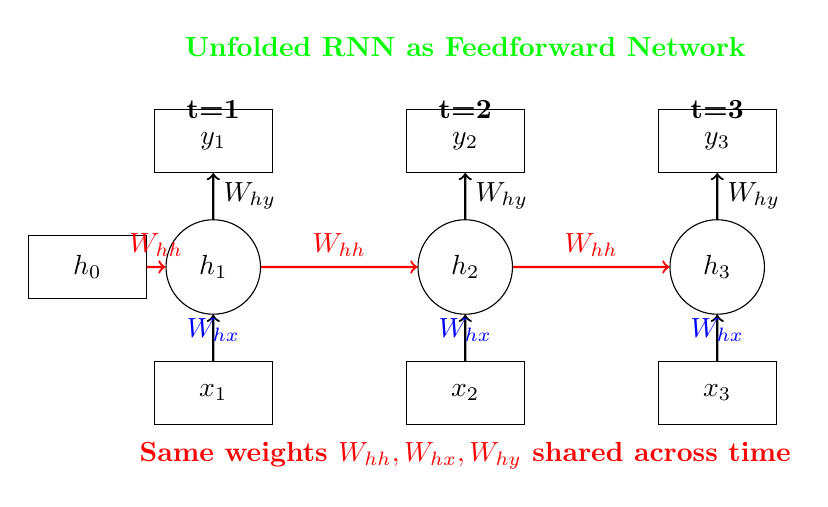
\begin{tikzpicture}[scale=0.8]
        % Time step labels
        \node at (2,6.5) {\textbf{t=1}};
        \node at (6,6.5) {\textbf{t=2}};
        \node at (10,6.5) {\textbf{t=3}};
        
        % Initial hidden state
        \node[draw, rectangle, minimum width=1.5cm, minimum height=0.8cm] (h0) at (0,4) {$h_0$};
        
        % Inputs
        \node[draw, rectangle, minimum width=1.5cm, minimum height=0.8cm] (x1) at (2,2) {$x_1$};
        \node[draw, rectangle, minimum width=1.5cm, minimum height=0.8cm] (x2) at (6,2) {$x_2$};
        \node[draw, rectangle, minimum width=1.5cm, minimum height=0.8cm] (x3) at (10,2) {$x_3$};
        
        % Hidden states
        \node[draw, circle, minimum size=1.2cm] (h1) at (2,4) {$h_1$};
        \node[draw, circle, minimum size=1.2cm] (h2) at (6,4) {$h_2$};
        \node[draw, circle, minimum size=1.2cm] (h3) at (10,4) {$h_3$};
        
        % Outputs
        \node[draw, rectangle, minimum width=1.5cm, minimum height=0.8cm] (y1) at (2,6) {$y_1$};
        \node[draw, rectangle, minimum width=1.5cm, minimum height=0.8cm] (y2) at (6,6) {$y_2$};
        \node[draw, rectangle, minimum width=1.5cm, minimum height=0.8cm] (y3) at (10,6) {$y_3$};
        
        % Input connections
        \draw[thick, ->] (x1) -- (h1);
        \draw[thick, ->] (x2) -- (h2);
        \draw[thick, ->] (x3) -- (h3);
        
        % Recurrent connections
        \draw[thick, red, ->] (h0) -- (h1) node[midway, above, red] {$W_{hh}$};
        \draw[thick, red, ->] (h1) -- (h2) node[midway, above, red] {$W_{hh}$};
        \draw[thick, red, ->] (h2) -- (h3) node[midway, above, red] {$W_{hh}$};
        
        % Output connections
        \draw[thick, ->] (h1) -- (y1) node[midway, right] {$W_{hy}$};
        \draw[thick, ->] (h2) -- (y2) node[midway, right] {$W_{hy}$};
        \draw[thick, ->] (h3) -- (y3) node[midway, right] {$W_{hy}$};
        
        % Weight sharing annotations
        \node[blue] at (2,3) {$W_{hx}$};
        \node[blue] at (6,3) {$W_{hx}$};
        \node[blue] at (10,3) {$W_{hx}$};
        
        % Labels
        \node[red] at (6,1) {\textbf{Same weights $W_{hh}, W_{hx}, W_{hy}$ shared across time}};
        \node[green] at (6,7.5) {\textbf{Unfolded RNN as Feedforward Network}};
    \end{tikzpicture}
    \end{center}
    
    \explanation{
    \textbf{RNN Unfolding Process:}
    
    \textbf{Original Recurrent Formulation:}
    \begin{align}
    h_t &= \tanh(W_{hx} x_t + W_{hh} h_{t-1} + b_h) \\
    y_t &= W_{hy} h_t + b_y
    \end{align}
    
    \textbf{Unfolded Equations for T=3:}
    \begin{align}
    h_1 &= \tanh(W_{hx} x_1 + W_{hh} h_0 + b_h) \\
    h_2 &= \tanh(W_{hx} x_2 + W_{hh} h_1 + b_h) \\
    h_3 &= \tanh(W_{hx} x_3 + W_{hh} h_2 + b_h) \\
    y_1 &= W_{hy} h_1 + b_y \\
    y_2 &= W_{hy} h_2 + b_y \\
    y_3 &= W_{hy} h_3 + b_y
    \end{align}
    
    \textbf{Key Properties of Unfolding:}
    
    \textbf{1. Weight Sharing Across Time:}
    \begin{itemize}
        \item Same $W_{hx}$ processes all inputs $x_1, x_2, x_3$
        \item Same $W_{hh}$ connects all hidden states
        \item Same $W_{hy}$ produces all outputs
        \item This sharing enables generalization across sequence positions
    \end{itemize}
    
    \textbf{2. Hidden State Connections:}
    \begin{itemize}
        \item Each $h_t$ depends on previous $h_{t-1}$ and current $x_t$
        \item Information flows left-to-right through hidden states
        \item Creates memory mechanism across time steps
        \item $h_3$ contains information from $x_1, x_2, x_3$ through recurrent connections
    \end{itemize}
    
    \textbf{3. Feedforward Network Equivalence:}
    \begin{itemize}
        \item Unfolded RNN becomes a feedforward network with shared weights
        \item Can apply standard backpropagation algorithm
        \item Each time step becomes a layer in feedforward network
        \item Enables gradient computation through time (BPTT)
    \end{itemize}
    
    \textbf{4. Variable Length Sequence Handling:}
    \begin{itemize}
        \item \textbf{Shorter sequences:} Simply stop unfolding earlier (T=2, T=1)
        \item \textbf{Longer sequences:} Continue unfolding for more time steps (T=4, T=5, ...)
        \item \textbf{Same weights:} $W_{hx}, W_{hh}, W_{hy}$ work for any sequence length
        \item \textbf{Dynamic computation:} Network adapts to input sequence length automatically
    \end{itemize}
    
    \textbf{Practical Implications:}
    \begin{itemize}
        \item Training uses BPTT on unfolded network
        \item Gradient flows backward through time from $h_3$ to $h_1$ to $h_0$
        \item Memory requirements scale with sequence length
        \item Longer sequences may cause vanishing gradient problems
    \end{itemize}
    }
    
    \item Discuss the Turing completeness of RNNs. Explain: \hfill (8 marks)
    \begin{itemize}
        \item What it means for RNNs to be Turing complete
        \item The role of recurrent connections in providing memory
        \item Difference between theoretical capacity and practical training
        \item Comparison with multilayer perceptrons as universal approximators
    \end{itemize}
    
    \answer{RNNs are Turing complete, meaning they can theoretically compute any computable function given sufficient time and precision, but practical limitations prevent achieving this theoretical capacity.}
    
    \explanation{
    \textbf{Turing Completeness Definition:}
    
    \textbf{What it means:}
    \begin{itemize}
        \item RNNs can simulate any Turing machine given sufficient resources
        \item Can compute any algorithmically computable function
        \item Equivalent computational power to general-purpose computers
        \item Can perform any computation that can be described algorithmically
    \end{itemize}
    
    \textbf{Theoretical Foundation:}
    \begin{itemize}
        \item Proven by Siegelmann \& Sontag (1995) for rational-weighted RNNs
        \item Even simple RNNs with proper weights can simulate Turing machines
        \item Requires only finite precision arithmetic (rational numbers)
    \end{itemize}
    
    \textbf{Role of Recurrent Connections in Memory:}
    
    \textbf{Memory Mechanism:}
    \begin{itemize}
        \item Hidden state $h_t$ serves as external memory tape
        \item Recurrent weights $W_{hh}$ implement read/write operations
        \item Information can be stored, retrieved, and modified over time
        \item Unbounded computation time allows unlimited memory access
    \end{itemize}
    
    \textbf{Computational Model:}
    \begin{itemize}
        \item \textbf{Input:} Sequence of symbols (like Turing machine tape)
        \item \textbf{Processing:} Hidden state transformations (like state transitions)
        \item \textbf{Memory:} Recurrent connections maintain information (like memory cells)
        \item \textbf{Output:} Generated sequences (like Turing machine output)
    \end{itemize}
    
    \textbf{Difference Between Theoretical and Practical:}
    
    \textbf{Theoretical Capacity:}
    \begin{itemize}
        \item Infinite precision arithmetic
        \item Unlimited sequence length
        \item Perfect weight optimization
        \item No numerical stability issues
    \end{itemize}
    
    \textbf{Practical Limitations:}
    \begin{itemize}
        \item \textbf{Finite Precision:} Floating-point arithmetic introduces errors
        \item \textbf{Vanishing Gradients:} Long sequences cause training difficulties
        \item \textbf{Limited Memory:} Hidden state size constrains memory capacity
        \item \textbf{Training Challenges:} Finding correct weights is computationally intractable
        \item \textbf{Sequence Length:} Practical sequences are finite and bounded
    \end{itemize}
    
    \textbf{Real-World Implications:}
    \begin{itemize}
        \item RNNs can learn complex algorithms but often fail to do so in practice
        \item Simple tasks like counting or copying can be challenging to learn
        \item Need architectural innovations (LSTM, attention) for practical success
    \end{itemize}
    
    \textbf{Comparison with MLPs as Universal Approximators:}
    
    \begin{tabular}{|p{5cm}|p{5cm}|}
    \hline
    \textbf{RNNs (Turing Complete)} & \textbf{MLPs (Universal Approximators)} \\
    \hline
    Can compute any algorithm & Can approximate any continuous function \\
    \hline
    Sequential, temporal processing & Static, feedforward processing \\
    \hline
    Unbounded computation time & Fixed computation time \\
    \hline
    Memory through recurrence & No memory mechanism \\
    \hline
    Dynamic input/output & Fixed input/output size \\
    \hline
    Can handle algorithms & Cannot handle algorithms requiring memory \\
    \hline
    \end{tabular}
    
    \textbf{Key Distinctions:}
    \begin{itemize}
        \item \textbf{MLPs:} Can approximate functions $f: \mathbb{R}^n \to \mathbb{R}^m$ (static mapping)
        \item \textbf{RNNs:} Can compute algorithms $f: \Sigma^* \to \Sigma^*$ (dynamic computation)
        \item \textbf{MLPs:} Limited to pattern recognition and regression
        \item \textbf{RNNs:} Can perform reasoning, counting, and algorithmic computation
    \end{itemize}
    
    \textbf{Practical Significance:}
    \begin{itemize}
        \item Turing completeness provides theoretical foundation for sequence modeling
        \item Explains why RNNs are suitable for algorithmic tasks
        \item Motivates research into making RNNs more practically capable
        \item Highlights importance of memory and sequential processing in AI
    \end{itemize}
    }
\end{enumerate}

\newpage
\paragraph{Question 6. RNN Training and Gradient Issues}\hfill (25 marks)\\
Based on RNN training theory and backpropagation through time.

\begin{enumerate}[(a)]
    \item Explain why hyperbolic tangent is preferred over ReLU in vanilla RNNs. Discuss: \hfill (8 marks)
    \begin{itemize}
        \item Need for bounded hidden state values
        \item Consistency of state representation across time
        \item Problems with unbounded activations in recurrent connections
        \item Trade-offs with gradient flow
    \end{itemize}
    
    \answer{Hyperbolic tangent is preferred in vanilla RNNs because it provides bounded outputs $[-1,1]$, preventing explosive growth in recurrent connections, though it contributes to vanishing gradients.}
    
    \explanation{
    \textbf{Need for Bounded Hidden State Values:}
    
    \textbf{Mathematical Analysis:}
    RNN hidden state update: $h_t = \tanh(W_{hx} x_t + W_{hh} h_{t-1} + b_h)$
    
    \textbf{With Tanh:}
    \begin{itemize}
        \item Output range: $h_t \in [-1, 1]$
        \item Bounded regardless of input magnitude
        \item Prevents hidden state explosion
        \item Provides numerical stability
    \end{itemize}
    
    \textbf{With ReLU:}
    \begin{itemize}
        \item Output range: $h_t \in [0, \infty)$
        \item Unbounded positive growth possible
        \item Can lead to explosive hidden states
        \item Numerical instability over time
    \end{itemize}
    
    \textbf{Consistency of State Representation:}
    
    \textbf{Tanh Advantages:}
    \begin{itemize}
        \item Symmetric around zero: $\tanh(-x) = -\tanh(x)$
        \item Consistent scale across all time steps
        \item Hidden states remain in predictable range
        \item Weights can be initialized to work with bounded inputs
    \end{itemize}
    
    \textbf{State Evolution Example:}
    \begin{itemize}
        \item $h_0 \in [-1, 1]$ (initial state)
        \item $h_1 = \tanh(\cdot) \in [-1, 1]$ (bounded)
        \item $h_2 = \tanh(\cdot) \in [-1, 1]$ (still bounded)
        \item Consistent representation maintained over time
    \end{itemize}
    
    \textbf{Problems with Unbounded Activations:}
    
    \textbf{ReLU in Recurrent Connections:}
    Consider: $h_t = \text{ReLU}(W_{hh} h_{t-1} + W_{hx} x_t + b)$
    
    \textbf{Exponential Growth Scenario:}
    \begin{itemize}
        \item If $W_{hh} > 1$ and inputs are positive
        \item $h_1 = \text{ReLU}(W_{hh} h_0 + \cdots) \geq W_{hh} h_0$
        \item $h_2 \geq W_{hh} h_1 \geq W_{hh}^2 h_0$
        \item $h_t \geq W_{hh}^t h_0$ (exponential growth)
    \end{itemize}
    
    \textbf{Consequences:}
    \begin{itemize}
        \item Hidden states can grow arbitrarily large
        \item Gradients become unstable
        \item Numerical overflow in practice
        \item Loss of information through saturation
    \end{itemize}
    
    \textbf{Trade-offs with Gradient Flow:}
    
    \textbf{Tanh Gradient Properties:}
    $$\frac{d}{dx}\tanh(x) = 1 - \tanh^2(x) \in (0, 1]$$
    
    \textbf{Advantages:}
    \begin{itemize}
        \item Non-zero gradients everywhere (no dead neurons)
        \item Smooth, continuous gradients
        \item Maximum gradient of 1 at $x = 0$
    \end{itemize}
    
    \textbf{Disadvantages:}
    \begin{itemize}
        \item Gradients approach 0 for large $|x|$ (vanishing gradient)
        \item Saturated activations stop learning
        \item Contributes to long-term dependency problems
    \end{itemize}
    
    \textbf{ReLU Gradient Properties:}
    $$\frac{d}{dx}\text{ReLU}(x) = \begin{cases} 1 & \text{if } x > 0 \\ 0 & \text{if } x \leq 0 \end{cases}$$
    
    \textbf{Advantages:}
    \begin{itemize}
        \item No vanishing gradient for positive activations
        \item Constant gradient of 1 in active region
        \item Promotes sparse representations
    \end{itemize}
    
    \textbf{Disadvantages in RNNs:}
    \begin{itemize}
        \item Dead neurons (gradient = 0) can kill information flow
        \item Unbounded activations cause instability
        \item Asymmetric activation disrupts recurrent dynamics
    \end{itemize}
    
    \textbf{Modern Solutions:}
    \begin{itemize}
        \item \textbf{LSTM/GRU:} Use gating to control information flow
        \item \textbf{Gradient Clipping:} Bound gradient magnitudes
        \item \textbf{Careful Initialization:} Control initial weight magnitudes
        \item \textbf{Residual Connections:} Add skip connections in deep RNNs
    \end{itemize}
    }
    
    \item For an RNN unfolded for 100 time steps, analyze the vanishing gradient problem: \hfill (12 marks)
    \begin{itemize}
        \item Why this creates a 100-layer feedforward network
        \item Mathematical explanation of gradient diminishing
        \item Effect of squashing activation functions
        \item Impact on learning long-term dependencies
    \end{itemize}
    
    Include analysis of gradient computation:
    $$\frac{\partial L}{\partial W_{hh}} = \sum_{t=1}^T \frac{\partial L_t}{\partial h_t} \frac{\partial h_t}{\partial W_{hh}}$$
    
    \answer{Unfolding creates a 100-layer network where gradients must flow backward through all layers, experiencing multiplicative decay through tanh derivatives, making learning of early dependencies nearly impossible.}
    
    \explanation{
    \textbf{100-Layer Feedforward Network Creation:}
    
    \textbf{Unfolding Process:}
    \begin{itemize}
        \item RNN unfolded for 100 time steps becomes 100-layer feedforward network
        \item Each time step corresponds to one layer
        \item Weights $W_{hh}, W_{hx}, W_{hy}$ are shared across all layers
        \item Information flows forward through layers: $h_1 \to h_2 \to \cdots \to h_{100}$
    \end{itemize}
    
    \textbf{Network Structure:}
    \begin{align}
    h_1 &= \tanh(W_{hx} x_1 + W_{hh} h_0) \\
    h_2 &= \tanh(W_{hx} x_2 + W_{hh} h_1) \\
    &\vdots \\
    h_{100} &= \tanh(W_{hx} x_{100} + W_{hh} h_{99})
    \end{align}
    
    \textbf{Mathematical Analysis of Gradient Diminishing:}
    
    \textbf{Full Gradient Computation:}
    $$\frac{\partial L}{\partial W_{hh}} = \sum_{t=1}^{100} \frac{\partial L_t}{\partial h_t} \frac{\partial h_t}{\partial W_{hh}}$$
    
    \textbf{Expanding $\frac{\partial h_t}{\partial W_{hh}}$ using chain rule:}
    $$\frac{\partial h_t}{\partial W_{hh}} = \frac{\partial h_t}{\partial h_{t-1}} \frac{\partial h_{t-1}}{\partial W_{hh}} + \frac{\partial h_t}{\partial W_{hh}}\bigg|_{\text{direct}}$$
    
    \textbf{For early time steps (e.g., $t=1$):}
    $$\frac{\partial h_{100}}{\partial h_1} = \prod_{k=2}^{100} \frac{\partial h_k}{\partial h_{k-1}} = \prod_{k=2}^{100} W_{hh} \cdot \tanh'(u_k)$$
    
    Where $u_k = W_{hx} x_k + W_{hh} h_{k-1} + b_h$
    
    \textbf{Gradient Magnitude Analysis:}
    $$\left|\frac{\partial h_{100}}{\partial h_1}\right| = \left|\prod_{k=2}^{100} W_{hh} \cdot \tanh'(u_k)\right| = |W_{hh}|^{99} \prod_{k=2}^{100} |\tanh'(u_k)|$$
    
    \textbf{Effect of Squashing Activation Functions:}
    
    \textbf{Tanh Derivative Properties:}
    \begin{itemize}
        \item $\tanh'(x) = 1 - \tanh^2(x) \in (0, 1]$
        \item Maximum value: $\tanh'(0) = 1$
        \item For most values: $\tanh'(x) < 1$
        \item Typical range in practice: $\tanh'(x) \in [0.1, 0.8]$
    \end{itemize}
    
    \textbf{Cumulative Effect:}
    \begin{itemize}
        \item Product of 99 terms each $< 1$
        \item Even with $\tanh'(x) = 0.5$ (optimistic): $(0.5)^{99} \approx 1.6 \times 10^{-30}$
        \item With typical values $\approx 0.3$: $(0.3)^{99} \approx 10^{-52}$
        \item Gradients become negligibly small
    \end{itemize}
    
    \textbf{Weight Matrix Contribution:}
    \begin{itemize}
        \item If $|W_{hh}| < 1$: $|W_{hh}|^{99}$ further diminishes gradient
        \item If $|W_{hh}| > 1$: Can lead to exploding gradients
        \item Sweet spot $|W_{hh}| \approx 1$ is difficult to maintain
    \end{itemize}
    
    \textbf{Impact on Learning Long-term Dependencies:}
    
    \textbf{Information Loss:}
    \begin{itemize}
        \item Gradient from $h_{100}$ to $h_1$ is $\approx 10^{-30}$ or smaller
        \item Weights receive virtually no learning signal from distant time steps
        \item Network cannot learn correlations between $x_1$ and $y_{100}$
    \end{itemize}
    
    \textbf{Practical Consequences:}
    \begin{itemize}
        \item \textbf{Short-term Memory Only:} RNN learns dependencies within ~10-20 time steps
        \item \textbf{Information Decay:} Older inputs have exponentially decreasing influence
        \item \textbf{Training Inefficiency:} Early layers receive weak gradients, learn slowly
        \item \textbf{Task Limitations:} Cannot solve problems requiring long-term memory
    \end{itemize}
    
    \textbf{Examples of Affected Tasks:}
    \begin{itemize}
        \item Language modeling: Cannot use context from beginning of long sentences
        \item Machine translation: Cannot align distant words in long sentences
        \item Time series: Cannot capture yearly patterns in daily data
        \item Algorithmic tasks: Cannot maintain counters or stack operations
    \end{itemize}
    
    \textbf{Mathematical Summary:}
    For learning dependency between $x_1$ and $y_{100}$:
    $$\frac{\partial L}{\partial W_{hh}} \propto \frac{\partial L}{\partial y_{100}} \frac{\partial y_{100}}{\partial h_{100}} \frac{\partial h_{100}}{\partial h_1} \frac{\partial h_1}{\partial W_{hh}}$$
    
    The term $\frac{\partial h_{100}}{\partial h_1} \approx 10^{-30}$ makes this gradient negligible, preventing learning.
    }
    
    \item Compare solutions to RNN gradient problems: \hfill (5 marks)
    \begin{itemize}
        \item Gradient clipping for exploding gradients
        \item Penalty terms for vanishing gradients
        \item When each approach is appropriate
    \end{itemize}
    
    \answer{Gradient clipping limits maximum gradient magnitude to prevent explosions; penalty terms and architectural solutions (LSTM, residual connections) address vanishing gradients; choice depends on which problem dominates.}
    
    \explanation{
    \textbf{Gradient Clipping for Exploding Gradients:}
    
    \textbf{Method:}
    \begin{itemize}
        \item Monitor gradient norm: $\|\nabla\| = \sqrt{\sum_i (\frac{\partial L}{\partial \theta_i})^2}$
        \item If $\|\nabla\| > \text{threshold}$: $\nabla \leftarrow \frac{\text{threshold}}{\|\nabla\|} \nabla$
        \item Preserves gradient direction, scales down magnitude
    \end{itemize}
    
    \textbf{Mathematical Formulation:}
    $$\tilde{\nabla} = \begin{cases} 
    \nabla & \text{if } \|\nabla\| \leq \tau \\
    \frac{\tau}{\|\nabla\|} \nabla & \text{if } \|\nabla\| > \tau
    \end{cases}$$
    
    \textbf{Advantages:}
    \begin{itemize}
        \item Simple to implement
        \item Effective for preventing training divergence
        \item Maintains gradient direction information
        \item Allows training of deeper RNNs
    \end{itemize}
    
    \textbf{Limitations:}
    \begin{itemize}
        \item Doesn't address vanishing gradients
        \item Threshold selection is crucial but difficult
        \item Can slow convergence if threshold too conservative
    \end{itemize}
    
    \textbf{Penalty Terms and Regularization for Vanishing Gradients:}
    
    \textbf{1. Gradient Penalty Methods:}
    \begin{itemize}
        \item Add terms to loss: $L' = L + \lambda \|\frac{\partial h_t}{\partial h_{t-k}}\|^2$
        \item Encourage gradients to maintain magnitude
        \item Directly optimize for better gradient flow
    \end{itemize}
    
    \textbf{2. Weight Regularization:}
    \begin{itemize}
        \item Encourage recurrent weights near identity: $L' = L + \lambda \|W_{hh} - I\|^2$
        \item Promotes gradient preservation
        \item Based on theory that identity matrix preserves gradients
    \end{itemize}
    
    \textbf{3. Spectral Regularization:}
    \begin{itemize}
        \item Control eigenvalues of $W_{hh}$: $L' = L + \lambda (\rho(W_{hh}) - 1)^2$
        \item $\rho(W_{hh})$ is spectral radius (largest eigenvalue magnitude)
        \item Keeps eigenvalues near 1 for stable gradients
    \end{itemize}
    
    \textbf{Architectural Solutions:}
    
    \textbf{1. LSTM/GRU:}
    \begin{itemize}
        \item Gating mechanisms control information flow
        \item Additive updates rather than multiplicative
        \item Dedicated memory pathways
    \end{itemize}
    
    \textbf{2. Residual Connections:}
    \begin{itemize}
        \item Add skip connections: $h_t = f(h_{t-1}, x_t) + h_{t-1}$
        \item Provides gradient highways
        \item Similar to ResNet for sequences
    \end{itemize}
    
    \textbf{When Each Approach is Appropriate:}
    
    \textbf{Gradient Clipping:}
    \begin{itemize}
        \item \textbf{When:} Training becomes unstable, loss oscillates wildly
        \item \textbf{Signs:} NaN values, exponentially growing loss
        \item \textbf{Best for:} Quick fix during training, debugging
        \item \textbf{Use with:} Any RNN architecture as safety measure
    \end{itemize}
    
    \textbf{Penalty Terms:}
    \begin{itemize}
        \item \textbf{When:} Research settings, when you want to keep vanilla RNN
        \item \textbf{Signs:} Poor long-term memory, gradients approach zero
        \item \textbf{Best for:} Understanding gradient behavior, proof-of-concept
        \item \textbf{Limitations:} Often less effective than architectural solutions
    \end{itemize}
    
    \textbf{Architectural Solutions (LSTM/GRU):}
    \begin{itemize}
        \item \textbf{When:} Production applications, need reliable long-term memory
        \item \textbf{Signs:} Penalty methods insufficient, complex sequence tasks
        \item \textbf{Best for:} Most practical applications
        \item \textbf{Trade-off:} More complex but much more effective
    \end{itemize}
    
    \textbf{Combined Approach (Recommended):}
    \begin{itemize}
        \item Use LSTM/GRU architecture
        \item Apply gradient clipping as safety measure
        \item Add residual connections for very deep networks
        \item Monitor gradient norms during training
    \end{itemize}
    }
\end{enumerate}

\newpage
\paragraph{Question 7. LSTM Architecture and Memory Mechanisms}\hfill (30 marks)\\
Based on LSTM theory and gating mechanisms for sequence modeling.

\begin{enumerate}[(a)]
    \item Design the complete LSTM architecture with mathematical equations. For input $x_t$, previous hidden state $h_{t-1}$, and previous cell state $C_{t-1}$, derive: \hfill (15 marks)
    
    \begin{itemize}
        \item Forget gate: $f_t = ?$
        \item Input gate: $i_t = ?$ 
        \item Candidate values: $\tilde{C}_t = ?$
        \item Cell state update: $C_t = ?$
        \item Output gate: $o_t = ?$
        \item Hidden state: $h_t = ?$
    \end{itemize}
    
    \answer{Complete LSTM equations with three gates controlling information flow through dedicated cell state pathway.}
    
    \explanation{
    \textbf{Complete LSTM Mathematical Formulation:}
    
    \textbf{1. Forget Gate:}
    $$f_t = \sigma(W_f \cdot [h_{t-1}, x_t] + b_f)$$
    
    \textbf{Purpose:} Decides what information to discard from cell state
    \begin{itemize}
        \item $f_t \in [0,1]$ for each dimension of cell state
        \item $f_t = 0$: completely forget old information
        \item $f_t = 1$: completely retain old information
        \item Sigmoid ensures values in $[0,1]$ range
    \end{itemize}
    
    \textbf{2. Input Gate:}
    $$i_t = \sigma(W_i \cdot [h_{t-1}, x_t] + b_i)$$
    
    \textbf{Purpose:} Decides which new information to store in cell state
    \begin{itemize}
        \item Controls which candidate values will be added
        \item $i_t \in [0,1]$ acts as importance weighting
        \item Works in conjunction with candidate values
    \end{itemize}
    
    \textbf{3. Candidate Values:}
    $$\tilde{C}_t = \tanh(W_C \cdot [h_{t-1}, x_t] + b_C)$$
    
    \textbf{Purpose:} Creates vector of new candidate values for cell state
    \begin{itemize}
        \item $\tilde{C}_t \in [-1,1]$ due to tanh activation
        \item Represents potential new information to be stored
        \item Modulated by input gate to determine actual contribution
    \end{itemize}
    
    \textbf{4. Cell State Update:}
    $$C_t = f_t \odot C_{t-1} + i_t \odot \tilde{C}_t$$
    
    \textbf{Purpose:} Updates cell state by forgetting old and adding new information
    \begin{itemize}
        \item $\odot$ denotes element-wise multiplication
        \item $f_t \odot C_{t-1}$: selectively retain old information
        \item $i_t \odot \tilde{C}_t$: selectively add new information
        \item Additive update prevents vanishing gradients
    \end{itemize}
    
    \textbf{5. Output Gate:}
    $$o_t = \sigma(W_o \cdot [h_{t-1}, x_t] + b_o)$$
    
    \textbf{Purpose:} Decides what parts of cell state to output as hidden state
    \begin{itemize}
        \item Controls which information is exposed to next time step
        \item $o_t \in [0,1]$ acts as filtering mechanism
        \item Allows internal memory to differ from external output
    \end{itemize}
    
    \textbf{6. Hidden State:}
    $$h_t = o_t \odot \tanh(C_t)$$
    
    \textbf{Purpose:} Produces final output based on filtered cell state
    \begin{itemize}
        \item $\tanh(C_t)$ squashes cell state to $[-1,1]$
        \item $o_t$ selectively filters this information
        \item $h_t$ becomes input to next time step and current output
    \end{itemize}
    
    \textbf{Parameter Dimensions:}
    For hidden size $h$ and input size $x$:
    \begin{itemize}
        \item $W_f, W_i, W_C, W_o \in \mathbb{R}^{h \times (h+x)}$
        \item $b_f, b_i, b_C, b_o \in \mathbb{R}^h$
        \item Total parameters: $4h(h+x) + 4h = 4h(h+x+1)$
    \end{itemize}
    
    \textbf{Information Flow Summary:}
    \begin{enumerate}
        \item Forget gate removes irrelevant information from $C_{t-1}$
        \item Input gate and candidates decide what new information to add
        \item Cell state combines retained and new information additively
        \item Output gate filters cell state for external use
        \item Hidden state provides processed information to next time step
    \end{enumerate}
    }
    
    \item Explain why LSTM solves the vanishing gradient problem. Focus on: \hfill (10 marks)
    \begin{itemize}
        \item Gradient flow through the cell state path
        \item Why $\frac{\partial C_t}{\partial C_{t-1}}$ doesn't involve squashing functions
        \item How this enables learning of long-term dependencies
        \item Mathematical comparison with vanilla RNN gradient flow
    \end{itemize}
    
    \answer{LSTM solves vanishing gradients through additive cell state updates where $\frac{\partial C_t}{\partial C_{t-1}} = f_t$, providing unimpeded gradient flow compared to vanilla RNN's multiplicative updates.}
    
    \explanation{
    \textbf{Gradient Flow Through Cell State Path:}
    
    \textbf{LSTM Cell State Update:}
    $$C_t = f_t \odot C_{t-1} + i_t \odot \tilde{C}_t$$
    
    \textbf{Gradient Computation:}
    $$\frac{\partial C_t}{\partial C_{t-1}} = f_t$$
    
    \textbf{Key Insight:} The gradient $\frac{\partial C_t}{\partial C_{t-1}} = f_t$ is controlled by the forget gate, not by activation function derivatives!
    
    \textbf{Why No Squashing Functions in Gradient Path:}
    
    \textbf{LSTM Advantage:}
    \begin{itemize}
        \item Cell state update is additive: $C_t = f_t \odot C_{t-1} + (\text{new info})$
        \item Gradient: $\frac{\partial C_t}{\partial C_{t-1}} = f_t$ (no activation derivative)
        \item $f_t \in [0,1]$ is learned, can be close to 1 when memory needed
        \item No forced multiplication by $\tanh'$ or similar derivatives
    \end{itemize}
    
    \textbf{Vanilla RNN Problem:}
    \begin{itemize}
        \item Hidden state update: $h_t = \tanh(W_{hh} h_{t-1} + W_{hx} x_t + b)$
        \item Gradient: $\frac{\partial h_t}{\partial h_{t-1}} = W_{hh} \odot \tanh'(\cdot)$
        \item Always includes $\tanh'(\cdot) \in (0,1]$ which typically $< 1$
        \item Forces gradient reduction at every time step
    \end{itemize}
    
    \textbf{Long-term Gradient Flow Analysis:}
    
    \textbf{LSTM Through Multiple Time Steps:}
    $$\frac{\partial C_T}{\partial C_1} = \prod_{t=2}^T \frac{\partial C_t}{\partial C_{t-1}} = \prod_{t=2}^T f_t$$
    
    \textbf{Gradient Preservation:}
    \begin{itemize}
        \item If $f_t \approx 1$ (forget gate learns to remember): $\frac{\partial C_T}{\partial C_1} \approx 1$
        \item Gradient magnitude preserved across time steps
        \item Network can choose when to forget ($f_t \approx 0$) vs. remember ($f_t \approx 1$)
        \item Learning determines optimal forget gate values
    \end{itemize}
    
    \textbf{Vanilla RNN Comparison:}
    $$\frac{\partial h_T}{\partial h_1} = \prod_{t=2}^T W_{hh} \odot \tanh'(u_t)$$
    
    \textbf{Forced Decay:}
    \begin{itemize}
        \item Each $\tanh'(u_t) \leq 1$, typically much less
        \item Product of many terms $< 1$ causes exponential decay
        \item No mechanism to prevent this decay
        \item Gradient vanishing is inevitable for long sequences
    \end{itemize}
    
    \textbf{Mathematical Comparison:}
    
    \begin{tabular}{|p{5.5cm}|p{5.5cm}|}
    \hline
    \textbf{LSTM} & \textbf{Vanilla RNN} \\
    \hline
    $\frac{\partial C_T}{\partial C_1} = \prod_{t=2}^T f_t$ & $\frac{\partial h_T}{\partial h_1} = \prod_{t=2}^T W_{hh} \tanh'(u_t)$ \\
    \hline
    $f_t$ is learned (can be $\approx 1$) & $\tanh'(u_t)$ is forced $< 1$ \\
    \hline
    Additive cell state updates & Multiplicative hidden state updates \\
    \hline
    Selective gradient flow control & No gradient flow control \\
    \hline
    Can maintain gradient magnitude & Gradient magnitude always decreases \\
    \hline
    \end{tabular}
    
    \textbf{Enabling Long-term Dependencies:}
    
    \textbf{1. Gradient Highway:}
    \begin{itemize}
        \item Cell state provides "highway" for gradients
        \item Gradients can flow back unimpeded when $f_t \approx 1$
        \item Learning signal reaches early time steps effectively
    \end{itemize}
    
    \textbf{2. Adaptive Memory:}
    \begin{itemize}
        \item Network learns when to remember vs. forget
        \item Important information maintained over long periods
        \item Irrelevant information discarded to make room for new data
    \end{itemize}
    
    \textbf{3. Practical Benefits:}
    \begin{itemize}
        \item Can learn dependencies spanning 100+ time steps
        \item Successful on tasks requiring long-term memory
        \item More stable training than vanilla RNNs
        \item Better performance on sequence modeling tasks
    \end{itemize}
    
    \textbf{Example Scenario:}
    For learning dependency between $x_1$ and $y_{100}$:
    \begin{itemize}
        \item \textbf{LSTM:} If important, forget gates learn $f_t \approx 1$ for $t = 2, \ldots, 100$
        \item \textbf{Result:} $\frac{\partial C_{100}}{\partial C_1} \approx 1$, strong gradient flow
        \item \textbf{Vanilla RNN:} $\frac{\partial h_{100}}{\partial h_1} \approx 0.5^{99} \approx 10^{-30}$, no learning
    \end{itemize}
    }
    
    \item Compare LSTM variants: \hfill (5 marks)
    \begin{itemize}
        \item LSTM with peephole connections
        \item Coupled forget and input gates
        \item GRU vs LSTM trade-offs
        \item When to choose each variant
    \end{itemize}
    
    \answer{LSTM variants offer different trade-offs: peephole connections add precision, coupled gates reduce parameters, GRU provides simplicity with comparable performance.}
    
    \explanation{
    \textbf{LSTM with Peephole Connections:}
    
    \textbf{Standard vs. Peephole LSTM:}
    
    \textbf{Standard:} Gates depend only on $h_{t-1}$ and $x_t$
    \textbf{Peephole:} Gates also depend on cell state $C_{t-1}$ (and $C_t$ for output gate)
    
    \textbf{Modified Equations:}
    \begin{align}
    f_t &= \sigma(W_f [h_{t-1}, x_t] + W_{pf} \odot C_{t-1} + b_f) \\
    i_t &= \sigma(W_i [h_{t-1}, x_t] + W_{pi} \odot C_{t-1} + b_i) \\
    o_t &= \sigma(W_o [h_{t-1}, x_t] + W_{po} \odot C_t + b_o)
    \end{align}
    
    \textbf{Advantages:}
    \begin{itemize}
        \item Gates can directly observe cell state information
        \item Better timing control for gate activations
        \item Can learn more precise gating decisions
        \item Useful for tasks requiring precise timing
    \end{itemize}
    
    \textbf{Disadvantages:}
    \begin{itemize}
        \item Additional parameters ($W_{pf}, W_{pi}, W_{po}$)
        \item Increased computational complexity
        \item Marginal performance improvement in most cases
    \end{itemize}
    
    \textbf{Coupled Forget and Input Gates:}
    
    \textbf{Motivation:} In many cases, when we forget old information, we should add new information (and vice versa)
    
    \textbf{Modified Equations:}
    \begin{align}
    f_t &= \sigma(W_f [h_{t-1}, x_t] + b_f) \\
    i_t &= 1 - f_t \\
    C_t &= f_t \odot C_{t-1} + (1-f_t) \odot \tilde{C}_t
    \end{align}
    
    \textbf{Advantages:}
    \begin{itemize}
        \item Reduces parameters (no separate input gate)
        \item Enforces complementary behavior
        \item Faster computation
        \item Often performs similarly to standard LSTM
    \end{itemize}
    
    \textbf{Disadvantages:}
    \begin{itemize}
        \item Less flexibility in gating decisions
        \item Cannot simultaneously retain old and add new information
        \item May be suboptimal for some tasks
    \end{itemize}
    
    \textbf{GRU vs LSTM Trade-offs:}
    
    \textbf{GRU Architecture:}
    \begin{align}
    r_t &= \sigma(W_r [h_{t-1}, x_t]) \quad \text{(reset gate)} \\
    z_t &= \sigma(W_z [h_{t-1}, x_t]) \quad \text{(update gate)} \\
    \tilde{h}_t &= \tanh(W_h [r_t \odot h_{t-1}, x_t]) \quad \text{(candidate)} \\
    h_t &= (1-z_t) \odot h_{t-1} + z_t \odot \tilde{h}_t
    \end{align}
    
    \textbf{Comparison Table:}
    
    \begin{tabular}{|p{3cm}|p{4cm}|p{4cm}|}
    \hline
    \textbf{Aspect} & \textbf{LSTM} & \textbf{GRU} \\
    \hline
    \textbf{Parameters} & $4h(h+x+1)$ & $3h(h+x+1)$ \\
    \hline
    \textbf{Gates} & 3 gates + cell state & 2 gates only \\
    \hline
    \textbf{Memory} & Separate cell state & Hidden state as memory \\
    \hline
    \textbf{Complexity} & Higher & Lower \\
    \hline
    \textbf{Training Speed} & Slower & Faster \\
    \hline
    \textbf{Performance} & Slightly better on complex tasks & Comparable on most tasks \\
    \hline
    \textbf{Gradient Flow} & Excellent (dedicated cell state) & Good (through hidden state) \\
    \hline
    \end{tabular}
    
    \textbf{When to Choose Each Variant:}
    
    \textbf{Standard LSTM:}
    \begin{itemize}
        \item \textbf{Use when:} Maximum performance needed, complex sequential tasks
        \item \textbf{Best for:} Language modeling, machine translation, complex time series
        \item \textbf{Advantages:} Most expressive, best long-term memory
        \item \textbf{Trade-offs:} Highest computational cost
    \end{itemize}
    
    \textbf{Peephole LSTM:}
    \begin{itemize}
        \item \textbf{Use when:} Precise timing is crucial, tasks with clear temporal patterns
        \item \textbf{Best for:} Speech recognition, music generation, periodic time series
        \item \textbf{Advantages:} Better temporal precision
        \item \textbf{Trade-offs:} More parameters, minimal performance gain
    \end{itemize}
    
    \textbf{Coupled Gates LSTM:}
    \begin{itemize}
        \item \textbf{Use when:} Want LSTM benefits with fewer parameters
        \item \textbf{Best for:} Resource-constrained environments, simpler tasks
        \item \textbf{Advantages:} Reduced parameters, enforced gate coupling
        \item \textbf{Trade-offs:} Less flexibility than standard LSTM
    \end{itemize}
    
    \textbf{GRU:}
    \begin{itemize}
        \item \textbf{Use when:} Good trade-off between performance and efficiency needed
        \item \textbf{Best for:} Most practical applications, real-time systems
        \item \textbf{Advantages:} Simpler, faster, comparable performance
        \item \textbf{Trade-offs:} Slightly less expressive than LSTM
    \end{itemize}
    
    \textbf{Decision Guidelines:}
    \begin{itemize}
        \item \textbf{Start with GRU:} Good default choice for most applications
        \item \textbf{Try LSTM:} If GRU performance insufficient for complex tasks
        \item \textbf{Consider peephole:} Only if timing precision is critical
        \item \textbf{Use coupled gates:} When parameter budget is tight
    \end{itemize}
    }
\end{enumerate}

\vfill
\begin{center}{\bf END OF PAPER}\end{center>
\end{document}